\documentclass{article}

\usepackage{graphicx}
\usepackage{tikz}
\usepackage{tikzsymbols}
\usetikzlibrary{calc,patterns,shapes.geometric}
\pagestyle{empty}
\usepackage[margin=0pt]{geometry}
\geometry{papersize={14in,12in}}

\def\centerarc[#1](#2)(#3:#4:#5){\draw[#1] ($(#2)+({#5*cos(#3)},{#5*sin(#3)})$) arc (#3:#4:#5);}

\begin{document}
	\begin{figure}
		\centering
		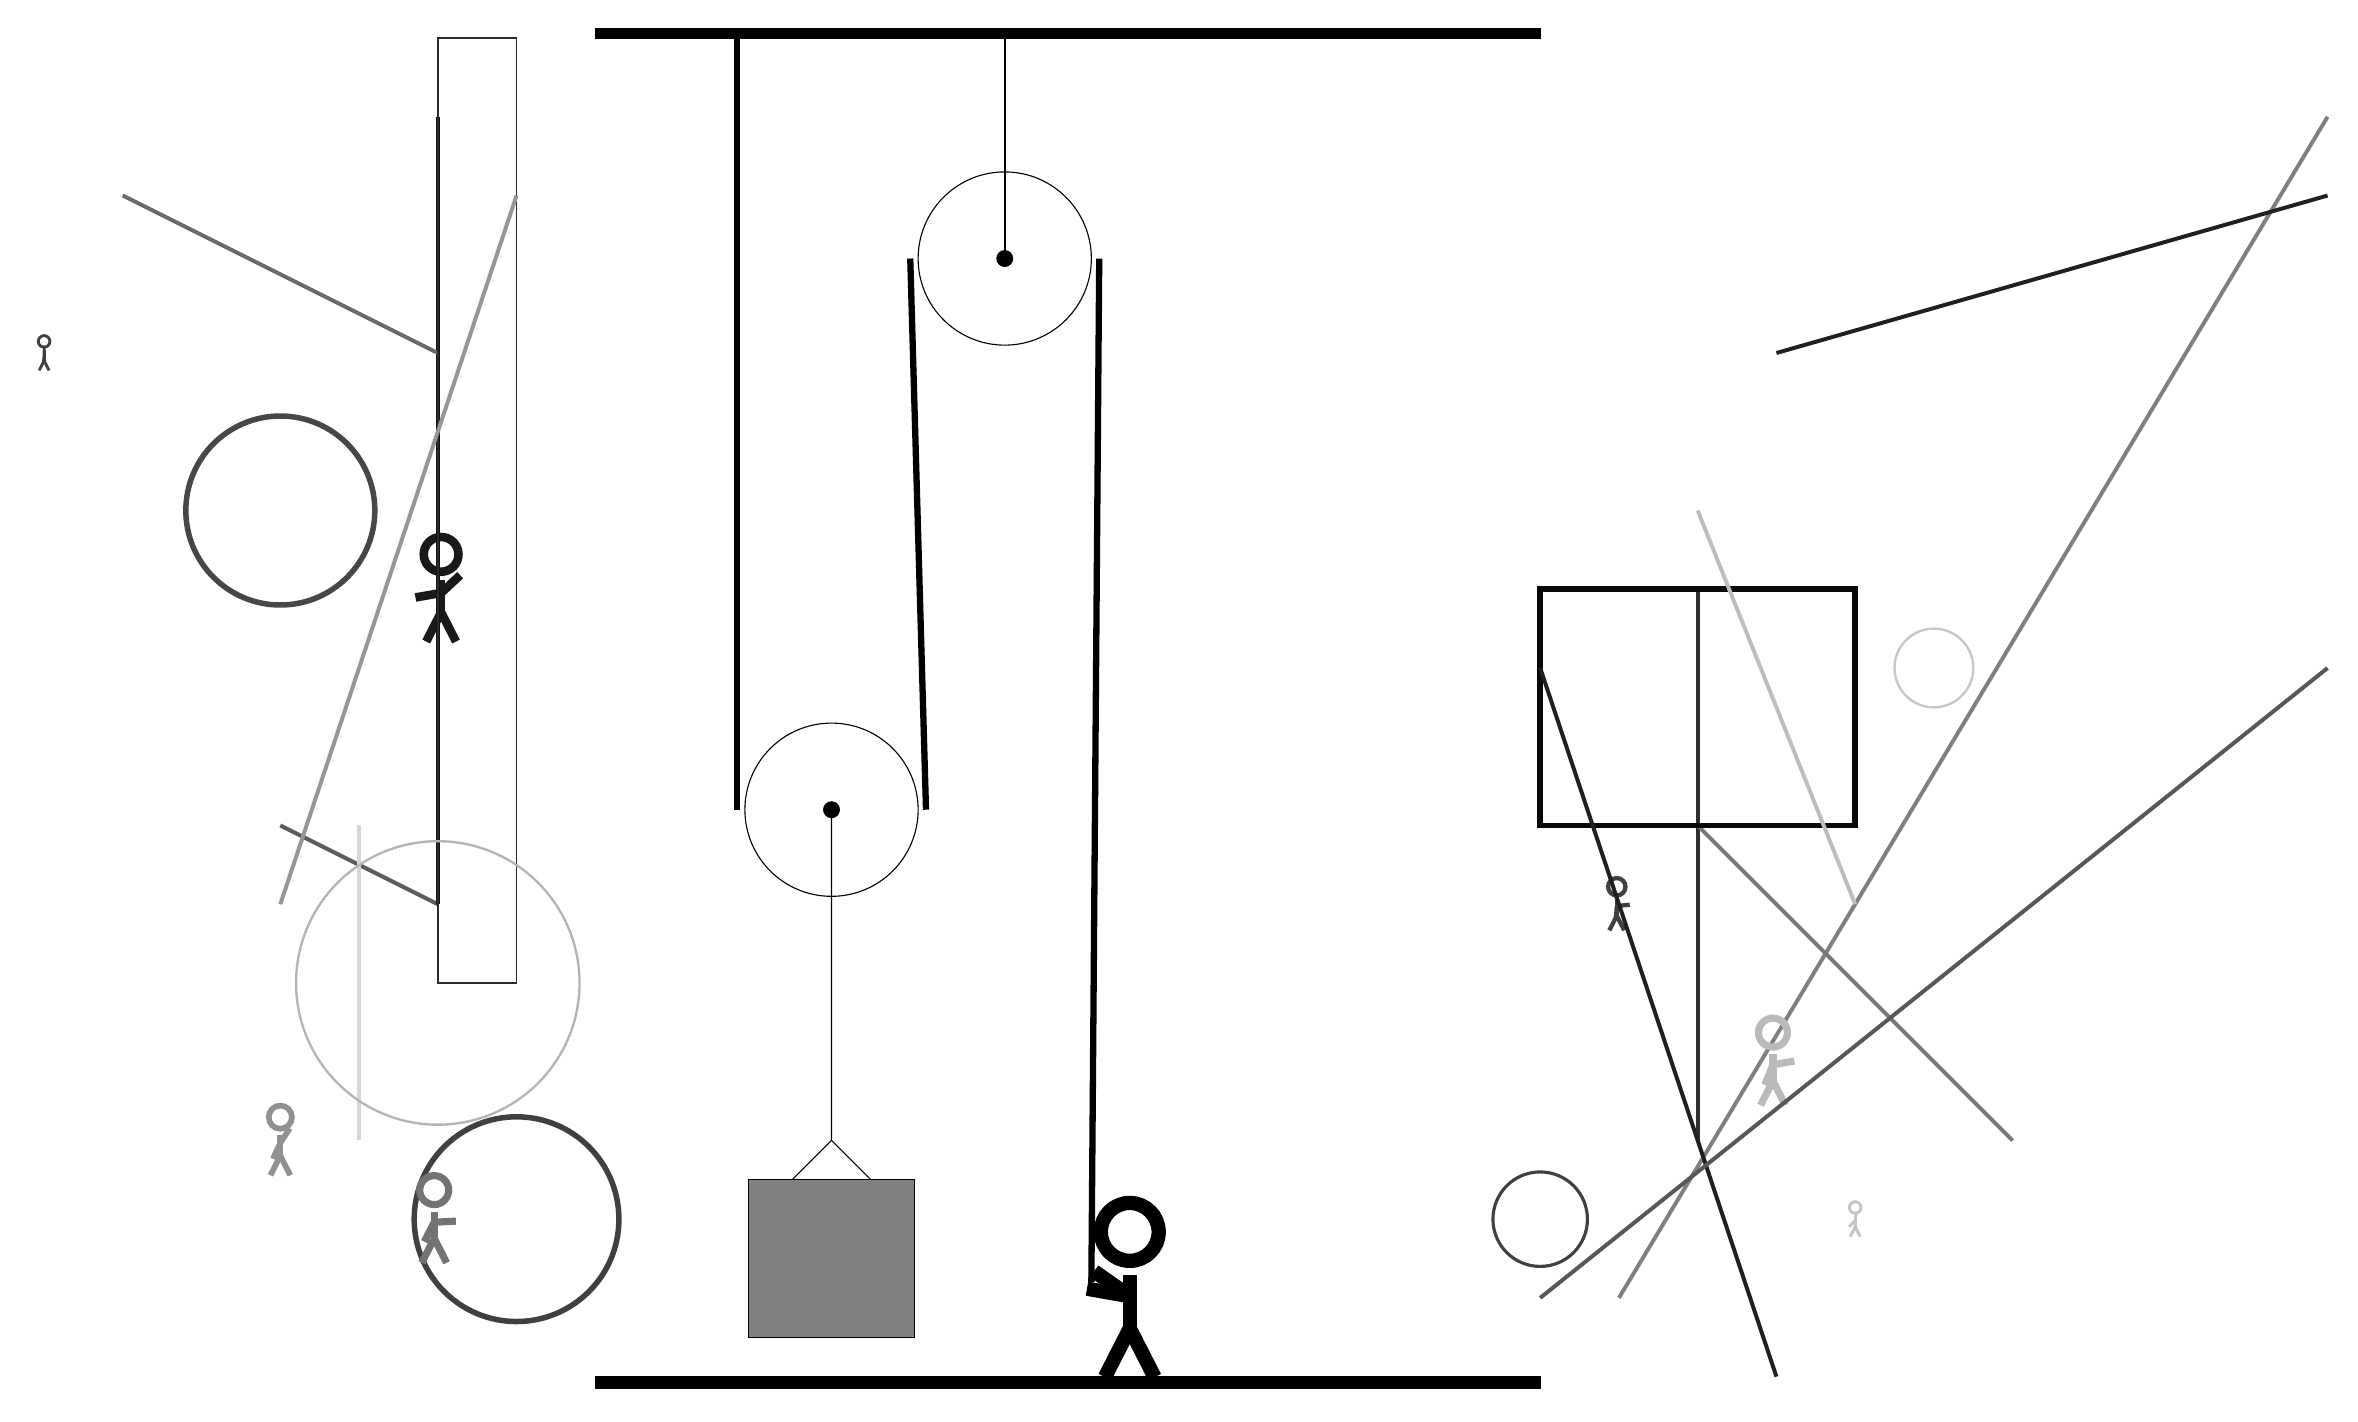
\begin{tikzpicture}
			%%%%% START %%%%%
			
			\draw[fill=black] (-2, 14) rectangle (10, 14.125);
			
			\draw[line width=0.5mm, color=black!50](11, -2) -- (20, 13);
			
			\draw [line width=0.3mm, color=black!22](15, 6) circle (0.5);
			\draw [line width=0.4mm, color=black!75](10, -1) circle (0.6);
			\draw[line width=0.5mm, color=black!87](13, 10) -- (20, 12);
			
			\draw[line width=0.5mm, color=black!64](-4, 3) -- (-6, 4);
			\node[line width=0.3mm, color=black!90] at (-4, 7) {\Strichmaxerl[6][10][43]};
			
			\node[line width=0.2mm, color=black!23] at (14, -1) {\Strichmaxerl[2][47][82]};
			
			\node[line width=0.3mm, color=black!75] at (11, 3) {\Strichmaxerl[3][86][6]};
			\node[line width=0.3mm, color=black!43] at (-6, 0) {\Strichmaxerl[4][65][57]};
			\draw[line width=0.5mm, color=black!82](12, 7) -- (12, 0);
			\draw [line width=0.7mm, color=black!72](-6, 8) circle (1.2);
			\draw[line width=0.5mm, color=black!53](12, 4) -- (16, 0);
			\node[line width=0.7mm, color=black!75] at (-9, 10) {\Strichmaxerl[2][85][89]};
			
			\draw [line width=0.7mm, color=black!75](-3, -1) circle (1.3);
			\draw[line width=0.5mm, color=black!93](-4, 13) -- (-4, 3);
			\draw[line width=0.5mm, color=black!16](-5, 4) -- (-5, 0);
			
			\draw[line width=0.7mm, color=black!97] (10, 4) rectangle (14, 7);
			\node[line width=0.5mm, color=black!27] at (13, 1) {\Strichmaxerl[5][68][10]};
			\draw[line width=0.5mm, color=black!59](-4, 10) -- (-8, 12);
			
			\draw[line width=0.5mm, color=black!88](13, -3) -- (10, 6);
			\draw[line width=0.2mm, color=black!83] (-3, 2) rectangle (-4, 14);
			\node[line width=0.7mm, color=black!55] at (-4, -1) {\Strichmaxerl[5][63][3]};
			\draw[line width=0.5mm, color=black!41](-3, 12) -- (-6, 3);
			\draw[line width=0.5mm, color=black!66](10, -2) -- (20, 6);
			\draw [line width=0.3mm, color=black!29](-4, 2) circle (1.8);
			
			\draw[line width=0.5mm, color=black!26](12, 8) -- (14, 3);
			
			
			\draw (3.2, 11.2) circle (1.1);
			\draw[fill=black] (3.2, 11.2) circle (0.1);
			\draw[thick] (3.2, 11.2) -- (3.2, 14);
			
			\draw (1, 4.2) circle (1.1);
			\draw[fill=black] (1, 4.2) circle (0.1);
			
			\draw (1, 4.2) -- (1, 0) -- (0.5, -0.5);
			\draw (1, 0) -- (1.5, -0.5);
			\draw[fill=black!50] (-0.05, -0.5) rectangle (2.05, -2.5);
			
			\draw[line width=0.8mm] (-0.2, 14) -- (-0.2, 4.2);
			\centerarc[line width=0.8mm](1, 4.2)(180:360:1.2000000000000002);
			\draw[line width=0.8mm](2.2, 4.2) -- (2.0, 11.2);
			\centerarc[line width=0.8mm](3.2, 11.2)(0:180:1.2000000000000002);
			\draw[line width=0.8mm](4.4, 11.2) -- (4.3, -1.8);
			
			\node at (4.7, -1.9) {\Strichmaxerl[10][-35][170]};
			
			\draw[fill=black] (-2, -3) rectangle (10, -3.15);
			
			%%%%% END %%%%%
		\end{tikzpicture}
	\end{figure}	
\end{document}